\section{DoS attack}

A DoS attack takes place when a client is used by the attacker to flood with TCP and UDP packets one target server overriding the resources of a system so that it cannot respond to service requests of legitimate users. This causes bandwidth saturation and the exhaustion of computing resources, even leading to a server crash.\\
A DDoS attack takes place when multiple systems target a single system with a DoS attack, more difficult to be tracked because the attack is launched by various positions.\\
Citing an example, one major use of IoT is home automation
systems. If an attacker attacks the main server of such a
system with a DoS attack, the whole system tends to shut
down and any appliance within the whole house (sometimes
even door locks) is made inaccessible. This small example
shows the significance of security implementation in IoT.
In IoT-based networks, new devices that enter the
network are configured automatically due to their open nature.
This leaves such networks prone to a lot of attacks. The open
nature of IoT makes it relatively easy for spammers and
attackers to infiltrate IoT networks and launch DoS attacks.

\subsection{Different type of Dos attack}
Unfortunately exist very different types of Dos attacks, based on the protocol that is used, if the aim is crash services or flood services. For example in a yo-yo attack, the attacker generates a flood of traffic until a cloud-hosted service scales outwards to handle the increase of traffic, then halts the attack, leaving the victim with over-provisioned resources. When the victim scales back down, the attack resumes, causing resources to scale back up again.
An example of a TCP attack is \textbf{SYN Flood Attack}. To better understand it we need a closer look at how TCP initializes a connection between a client and a server.

The algorithm used by TCP to establish and terminate a connection is called a three-way handshake.
The idea is that two parties want to agree on a set of parameters, which, in the case of opening a TCP connection, are the starting sequence numbers the two sides plan to use for their respective byte streams. In general, the parameters might be any facts that each side wants the other to know about. First, the client (the active participant) sends a segment to the server (the passive participant) stating the initial sequence number it plans to use (Flags = SYN, SequenceNum = x). The server then responds with a single segment that both acknowledges the client's sequence number (Flags = ACK, Ack = x + 1) and states its own beginning sequence number (Flags = SYN, SequenceNum = y). That is, both the SYN and ACK bits are set in the Flags field of this second message. Finally, the client responds with a third segment that acknowledges the server's sequence number (Flags = ACK, Ack = y + 1). The reason why each side acknowledges a sequence number that is one larger than the one sent is that the Acknowledgment field actually identifies the “next sequence number expected,” thereby implicitly acknowledging all earlier sequence numbers.
To better understand the step to establish the connection, please refer to the figure below.
\begin{figure}[h!]
\centering
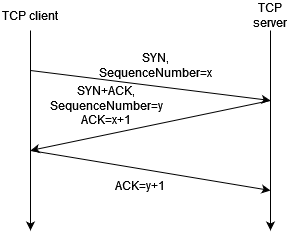
\includegraphics[width = 10cm]{images/TCP3wayHANDSHAKE.drawio.png}
\caption{TCP handshake protocol}
\label{fig:TCP}
\end{figure}
\FloatBarrier
\noindent

An attacker that wants to establish a \textbf{SYN Flood Attack} creates a bot that creates thousands of first segments in the 3-way handshake protocol. Then when the server replies with the SYN-ACK packet, the bot client never reply to it to make thousands of incomplete request of connection to the server to slow down it. Please refer to the picture below.

\begin{figure}[h!]
\centering
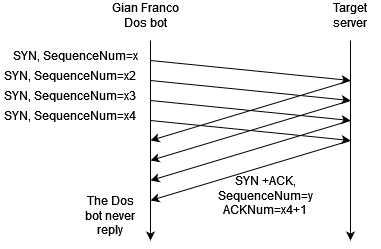
\includegraphics[width = 10cm]{images/DosSYNFloodAttack.drawio.png}
\caption{TCP SYN flood attack}
\label{fig:TCPDos}
\end{figure}
\FloatBarrier
\noindent
Now, the following question is, could we use honeypots to avoid this type of TCP attack?
According to what we found on the internet, to protect our servers from the \textbf{SYN Flood Attack}, is better to:
\begin{itemize}
\item Installing an IPS to detect anomalous traffic patterns;
\item configure the onsite firewall for SYN Attack Thresholds and SYN Flood protection;
\item Installing up-to-date networking equipment that has rate-limiting capabilities.
\end{itemize}
So honeypots are not useful to prevent that.